\section{Background and Problem Formulation}\label{sec:problem}
%% Planning Model Figure
\begin{figure}[t!]
    \begin{subfigure}{1.0\hsize}
         \centering    
         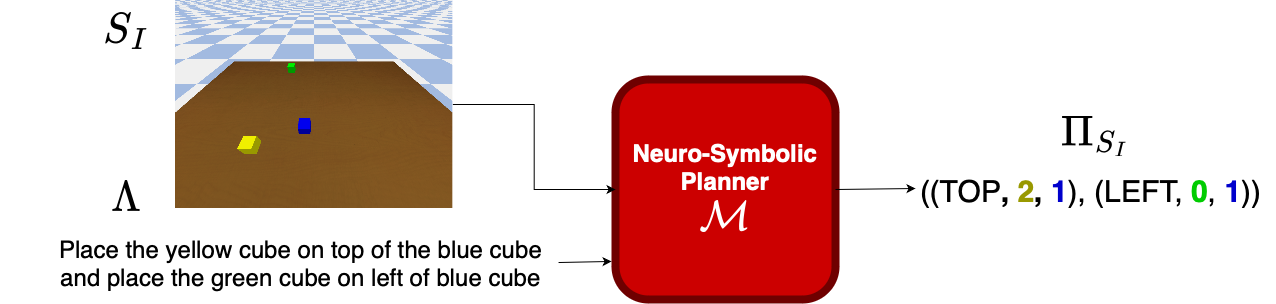
\includegraphics[scale=0.25]{figures/nsrm.png}
    \end{subfigure}
    \caption{
        \footnotesize{
            \textbf{Planning model.} 
            This work assumes a planning model that given a language utterance and the current world state can synthesize a sequence of actions for manipulation tasks. Crucially, the actions (as well as spatial relations) are functions that can be trained from goal-reaching human task demonstrations. 
        }
    }
    \vspace{-0.15in}
    \label{fig:nsrm}
\end{figure}


\textbf{Robot Model. }
Consider a robot manipulator capable of grasping and releasing objects in a table-top workspace. 
%
The robot can be tasked with instructions such as ``place the green block on top of the red object and the yellow block on top of the green one" that require the robot to sequentially manipulate objects to achieve an intended block assembly. 
%
We assume that the robot perceives the world through the visual sensor and is equipped with a primitive skill for grasping a specified object and releasing it at a given pose on the table or on another object. 
%
Further, we assume the presence of a planning model, $\mathcal{M}$, which given an initial world state $S_I$ and a goal specified as a language utterance $\mathit{\Lambda}$, can synthesise a plan $\mathbf{\Pi_{S_I}}$ for the robot to execute. 
%
Here, the plan $\Pi \in \mathcal{P}$ is a sequence of $T$ symbolic actions $\Pi = (\pi_1, \pi_2, .., \pi_T)$. The state $S_I$ is assumed to be represented as a set of bounding boxes extracted from a visual and depth sensor using a pre-trained object detection model. 

%
\textbf{Planning Model. }
%
We build on~\citep{Kalithasan2022LearningNP}, a contemporary neuro-symbolic planner that can learn grounded models for spatial concepts (left, right, on top etc.) as well as actions (e.g, moving an object to a prescribed location). 
%
The planner (Figure~\ref{fig:nsrm}) outputs a sequence of triplets ($a_t$, $o_{1t}$, $o_{2t}$), where $a_t$ is the symbolic action and, $o_{1t}$ and $o_{2t}$ are the indices of the \textit{subject} and \textit{object} of the manipulation task respectively. 
%
The predicted state changes by executing a plan $\mathbf{\Pi} \in \mathcal{P}$ on the state $S \in \mathcal{S}$ is modeled as a function, $\mathcal{E}: \mathcal{S} \times \mathcal{P} \rightarrow \mathcal{S}$. 
%
Further, let $\mathcal{K}: \mathcal{S} \times \mathcal{A} \rightarrow \mathcal{S}$, denote the \emph{transition model} that determines the state resulting from taking an action in a given state under nominal conditions (without errors). The transition model  $\mathcal{K}$ expresses the function $\mathcal{E}$ as follows where the state $\mathcal{E}(S, \mathbf{\Pi})$ will be reached if the plan is executed by the robot without any errors. 
%
\begin{equation}
    \mathcal{E}(S, \Pi) = \mathcal{E}(\mathcal{K}(S, \pi_1), (\pi_2, \pi_3, \dots, \pi_T)),
\end{equation}

% ROLL OUT FIGURE
\begin{figure}[t!]
    \begin{subfigure}{1.0\hsize}
         \centering    
         \includegraphics[scale=0.19]{figures/demo.png}
    \end{subfigure}
    \caption{
        \footnotesize{
            \textbf{Error detection and recovery pipeline.}
            Figure illustrates our error detection and recovery pipeline. Using the scene-graph predictor, we can \textit{imagine} the intermediate states that the robot should encounter during manipulation. We compare those with the actual state at run-time (at each step) and detect discrepancies if any. In case of discrepancy, our recovery mechanism kicks in and a plan is generated to the \textit{imagined} state. 
        }
    }
    \vspace{-0.15in}
    \label{fig:rollout}
\end{figure}

\textbf{Learning to Recover Plans. }
%
Online plan execution may be prone to \emph{internal} or \emph{external} disturbances, causing the robot to be in an \emph{unplanned} erroneous intermediate state, $S_E$. Hence, the robot may find itself in intermediate states to be different than the ones expected $S_t$ due to disturbances which necessitates the synthesis of a new \emph{recovery} plan $\mathbf{\Pi_{S_E}}$, such that $\mathcal{E}(S_E, \mathbf{\Pi_{S_E}}) =_\mathcal{S} \mathcal{E}(S_I, \mathbf{\Pi_{S_I}})$, see Figure~\ref{fig:rollout}.
%
Formally, for each $t \leq T$, we inductively define $S_t = \mathcal{K}(S_{t - 1}, \pi_t)$, where $S_0$ is the initial state. These $S_t$'s represent the \emph{intended} intermediate states for the robot. Further, let the states encountered during \emph{actual} execution be $S'_t$, $t \leq T$. 
%
The relation $=_\mathcal{S}$ on $\mathcal{S}$ holds if and only if the 3D positions of the corresponding objects in the two states are within some $\delta$ threshold. 
%
A plan recovery model requires addressing the following. First, estimating if there is a plan error (or discrepancy) as whether $S'_t =_\mathcal{S} S_t$ before executing action $\pi_{t + 1}$, for all plan execution steps $t$. 
%
Second, if a discrepancy is estimated, then synthesize a plan $\mathbf{\Pi_{E(t)}}$ such that $\mathcal{E}(S'_t, \mathbf{\Pi_{E(t)}}) =_\mathcal{S} S_k$ for some $k \leq T$.
%
Further, append the sequence $(\pi_{k + 1}, \pi_{k + 2}, .., \pi_T)$ to $\Pi_{E(t)}$ to get the overall plan $\Pi_{S_t'}$, such that $\mathcal{E}(S_t', \Pi_{S_t'}) =_\mathcal{S} S_T$. 
